\documentclass[]{article}
\usepackage{tikz}
\usepackage{listings}


%opening
\title{Theoretical simulation method for micro economic behaviour}
\author{3384257975982496768}


\begin{document}

\maketitle
\newpage

%\begin{abstract}
%\end{abstract}


\section{Economic fundamental re-framing}

\subsection{Assumptions}

My realisations, listed below will serve as the building block of all other analysis. Assuming that they are true and that the underlying reason is sound. 

Efficiently: typically in engineering no system can have an efficiency of more than 1, however in this context the $e$ acts as a coefficient of the $(\delta v output) / ( \delta v input)$. As sometimes storing things can add to the value it is possible to get more pleasure from it than was put in.

That there are only labour costs and nothing else. For example take any product or service, the price is defined as only the total of all labour coast associated with the product. in manufacturing a product is often broken down into labour costs and non-labour costs. Non-lobar costs often include materials, parts, tools, tool ware, tool depreciation and transport costs. I would like to assert that this may be true of the current level of manufacturing but not true when considering all layers of production. from example a product that is the comprised of a raw material and labour can be expressed as the sum of the labour of that processes as well as the labour involved in extracting and transporting the raw material. 

All claims made with respect to trading assume a free market.

\subsection{Definition of $\rho$, $\varphi$, $P$}
%can also do \subsubsection{Title}

at a fundamental level human interaction can be ranked on a scale of pleasure and pain. Henceforth denoted as $\rho$. This can be used to describe the pleasure of an event at an instant in time. similar to the concept of black body radiation the idea of there being a value of $\rho$ is absolute and is the identical scale between people. What does not remain constant is that two people may have two values of $\rho$ for the same activity as it's level of effect varies subjectively \\
\begin{figure}[!h]
	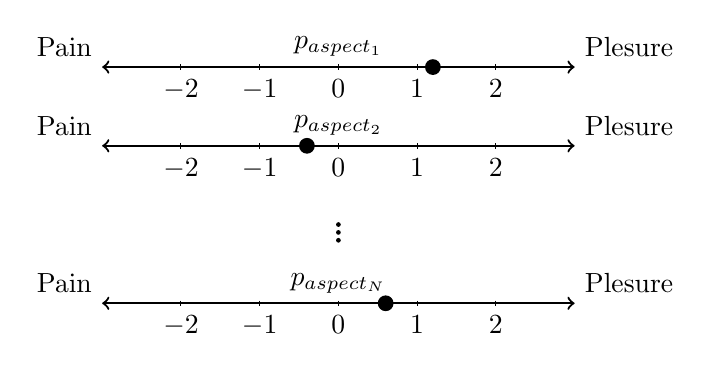
\begin{tikzpicture}
		\draw[thick] (0,1) -- (0,1) node[anchor=south]{$p_{aspect_{1}}$};
		\draw[thick,->] (0,1) -- (-3,1) node[anchor=south east]{Pain};
		\draw[thick,->] (0,1) -- (3,1) node[anchor=south west]{Plesure};
		\foreach \x in {-2,-1,0,1,2}
			\draw (\x cm,1pt + 1 cm) -- (\x cm,-1pt + 1 cm) node[anchor=north] {$\x$};
		\fill[black] (1.2, 1) circle (1mm);
		
		\draw[thick] (0,0) -- (0,0) node[anchor=south]{$p_{aspect_{2}}$};
		\draw[thick,->] (0,0) -- (-3,0) node[anchor=south east]{Pain};
		\draw[thick,->] (0,0) -- (3,0) node[anchor=south west]{Plesure};
		\foreach \x in {-2,-1,0,1,2}
			\draw (\x cm,1pt) -- (\x cm,-1pt) node[anchor=north] {$\x$};
		\fill[black] (-0.4,0) circle (1mm);
		
		\foreach \x in { 0, -0.1, -0.2}
			\fill[black] (0, \x - 1) circle (0.3mm);
			
		\draw[thick] (0,-2) -- (0,-2) node[anchor=south]{$p_{aspect_{N}}$};
		\draw[thick,->] (0,-2) -- (-3,-2) node[anchor=south east]{Pain};
		\draw[thick,->] (0,-2) -- (3,-2) node[anchor=south west]{Plesure};
		\foreach \x in {-2,-1,0,1,2}
			\draw (\x cm,1pt -2 cm) -- (\x cm,-1pt -2 cm) node[anchor=north] {$\x$};
	\fill[black] (0.6, -2) circle (1mm);
	\end{tikzpicture}
	\centering
\end{figure}
\\
The total of all pleasure and pain that an individual is experiencing at any one time is $P$ where:
\begin{equation}\label{Pdef}
	P = \sum \rho
\end{equation}
A scale of attributed pleasure value $\rho$ integrated over the time of an activity can be defined as the sum of the integrated change in pleasure with respect to that activity:
\begin{equation}\label{phidef}
	\varphi = \sum{\int{ \Delta \rho  \:  dt }}
\end{equation}
This can be thought of as a fundamental store input of value. Not necessarily the output of value ether. Since the exact scale of value for each individual is not represented in a standardised format translatable to another The effective of 'value' ($\varphi$). An efficient can only be meaningful in the context of the individual's 'value' spent to that of the potential 'value' returned.
\begin{equation}
	\eta = \frac{\varphi_{potentualOutput}}{\varphi_{input}} 
\end{equation} 
This value is not limited to the traditional domain of $\left\lceil 0, 1 \right\rceil $, instead being capable of residing at $>1$.



\subsection{Individual trade-off}
An individual will (generally) opt to choose the option at any time that is has the most $\varphi$, such as doing option $a$ or not doing option $a$. When ignoring time delay factors a trade for $a$ can be expressed as:
\begin{equation}\label{ind_trd}
	\varphi_{option} > \varphi_{alternative}
\end{equation}
However when time difference is relevant, the pleasure and pain become subject to the expected or anticipated $\varphi$. Notice that the factors subject to time also has an effect in relation to the decision to make a trade.
\begin{equation}\label{ind_trd_tm}
	\varphi_{anticipated} + \varphi_{timeSubdugation} > \varphi_{alternative}
\end{equation}


\subsection{Exchanges}
The first assumption that must be made here is that the individual scaling of $\rho$ remain independent from both parties exchanging any form of effort. If person one ($p1$) and person two ($p2$) each \textit{perceive} the exchange as being the higher $\varphi$ it in therefore deemed in each of their own individual interests.
\begin{equation}\label{trade_def}
	(\varphi_{p1, trade} > \varphi_{p1, noTrade}) \cup (\varphi_{p2, trade} > \varphi_{p2, noTrade})
\end{equation}\\
when given options of trades people will choose the option that has the highest increment of $\varphi$
\begin{equation}\label{trade_chc}
	rows
\end{equation}


\end{document}


word graveyard

The distinction between the local coordinate $p$ and the global coordinate $P$ can be made by overlaying the scales of each individual definition of $p$ to the global scale for an activity. 



that relative value $\varphi$ can be defined numerically as the integral of  potential $p$ over time. where negative numbers represented discomfort two distinctions can be made. first that there is the $\varphi$' that is apparent from the amount of value that has gone into an activity. the second, the amount of value that has been saved by acquiring 'v' value. 'delta



the range of this scales $\left\lceil - \infty, \infty \right\rceil $. Where activities can have a $p$ value that changes over time. Due to how humans perceive meaning moralistically, an arbitrary scale can be assignment to this dimension as the most meaningful or pleasurable things will 'resize' the scale
